\subsection{Другие объекты}
\begin{minipage}{0.63\tw}
\term{Шаровое звёздное скопление}~--- скопление звёзд, состоящее из нескольких сотен тысяч светил, тесно связанных гравитацией. Млечный путь насчитывает около 160 шаровых звёздных скоплений. Диаметры шаровых скоплений составляют 20\,--\,60~пк, массы~--- $10^4$\,--\,$10^6$~солнечных.\par

\term{Планетарная туманность}~--- система из звезды, называемой ядром туманности, и симметрично окружающей ее светящейся газовой оболочки. Планетарные туманности образуются при сбросе внешних слоёв (оболочек) красных гигантов и сверхгигантов с массой от $0.8M_\odot$ до $8M_\odot$ на завершающей стадии их эволюции. Характерный размер~--- 1\,--\,2~св.\,лет.
\end{minipage}
\hfill
\begin{minipage}{0.32\tw}
	\centering
	\vspace{-1.2pc}
	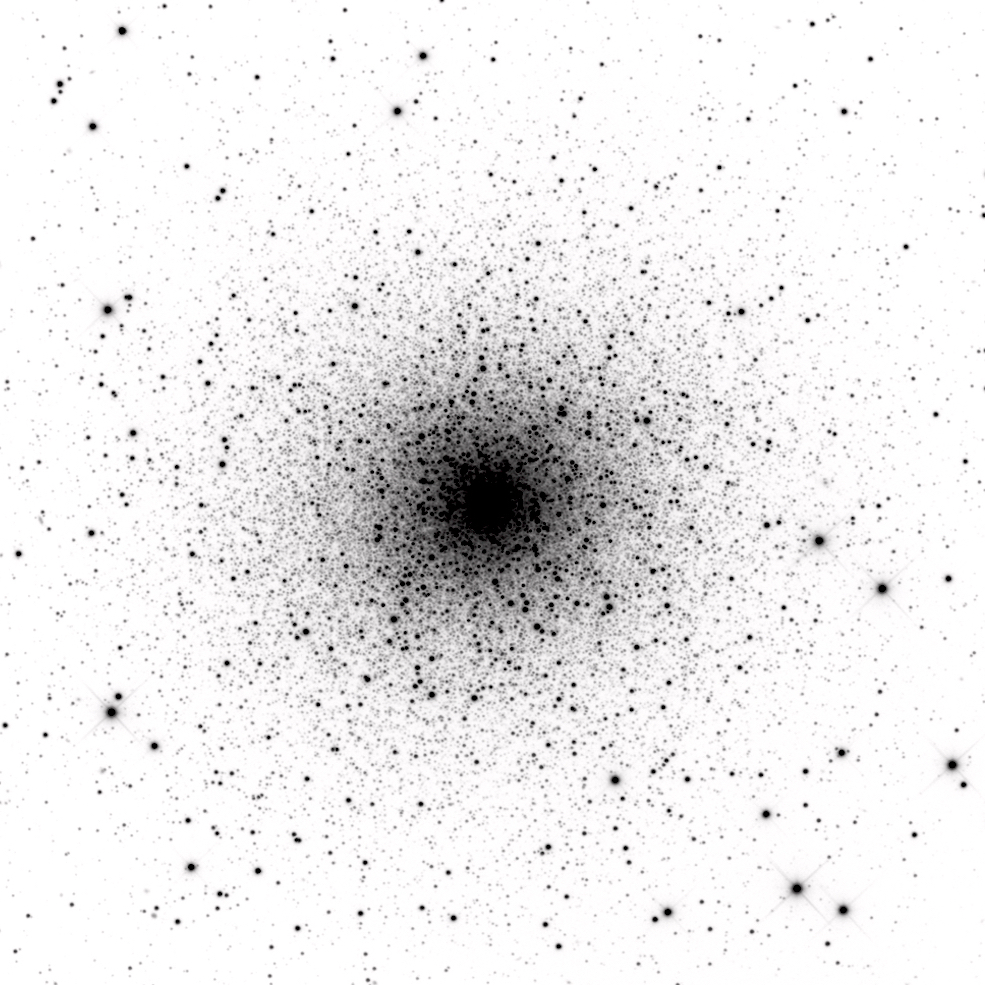
\includegraphics[width = .55\tw]{m13}
	\captionof{figure}{Шаровое скопление M13 (негатив)}
	\vspace{1pc}
	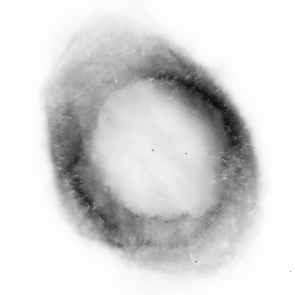
\includegraphics[width = .55\tw]{m57}
	\captionof{figure}{Пла\-не\-тар\-ная туманность M57 (негатив)}
\end{minipage}